%!TEX program = xelatex
%%%%%%%%%%%%%%%%%%%%%%%%%%%%%%%%%%%%%%%%%
% Short Sectioned Assignment
% LaTeX Template
% Version 1.0 (5/5/12)
%
% This template has been downloaded from:
% http://www.LaTeXTemplates.com
%
% Original author:
% Frits Wenneker (http://www.howtotex.com)
%
% License:
% CC BY-NC-SA 3.0 (http://creativecommons.org/licenses/by-nc-sa/3.0/)
%
%%%%%%%%%%%%%%%%%%%%%%%%%%%%%%%%%%%%%%%%%

%----------------------------------------------------------------------------------------
%	PACKAGES AND OTHER DOCUMENT CONFIGURATIONS
%----------------------------------------------------------------------------------------

\documentclass[paper=a4, fontsize=11pt]{scrartcl} % A4 paper and 11pt font size
\usepackage{xeCJK}
\usepackage{subfigure}
\usepackage{gensymb}
\usepackage{float}
\usepackage[T1]{fontenc} % Use 8-bit encoding that has 256 glyphs
\usepackage{fourier} % Use the Adobe Utopia font for the document - comment This line to return to the LaTeX default
\usepackage[english]{babel} % English language/hyphenation
\usepackage{amsmath,amsfonts,amsthm} % Math packages
\usepackage{graphicx}
\usepackage{lipsum} % Used for inserting dummy 'Lorem ipsum' text into the template
\usepackage{enumerate}
\usepackage{sectsty} % Allows customizing section commands
\allsectionsfont{\normalfont\scshape} % Make all sections centered, the default font and small caps

\usepackage{fancyhdr} % Custom headers and footers
\pagestyle{fancyplain} % Makes all pages in the document conform to the custom headers and footers
\fancyhead{} % No page header - if you want one, create it in the same way as the footers below
\fancyfoot[L]{} % Empty left footer
\fancyfoot[C]{} % Empty center footer
\fancyfoot[R]{\thepage} % Page numbering for right footer
\renewcommand{\headrulewidth}{0pt} % Remove header underlines
\renewcommand{\footrulewidth}{0pt} % Remove footer underlines
\setlength{\headheight}{13.6pt} % Customize the height of the header
\numberwithin{equation}{section} % Number equations within sections (i.e. 1.1, 1.2, 2.1, 2.2 instead of 1, 2, 3, 4)
\numberwithin{figure}{section} % Number figures within sections (i.e. 1.1, 1.2, 2.1, 2.2 instead of 1, 2, 3, 4)
\numberwithin{table}{section} % Number tables within sections (i.e. 1.1, 1.2, 2.1, 2.2 instead of 1, 2, 3, 4)

\setlength\parindent{2em} % Removes all indentation from paragraphs - comment this line for an assignment with lots of text

%----------------------------------------------------------------------------------------
%	TITLE SECTION
%----------------------------------------------------------------------------------------

\newcommand{\horrule}[1]{\rule{\linewidth}{#1}} % Create horizontal rule command with 1 argument of height

\title{	
\normalfont \normalsize 
\textsc{Zhiyuan College, Shanghai Jiaotong University} \\ % Your university, school and/or department name(s)
\horrule{0.5pt} \\[0.4cm] % Thin top horizontal rule
\huge CS389: Foundations of Data Science Homework IV\\ % The assignment title
\horrule{2pt} \\ % Thick bottom horizontal rule
}

\author{Zihao Ye} % Your name

\date{\normalsize\today} % Today's date or a custom date

\begin{document}

\maketitle % Print the title

\section*{exercise 5.9}
\begin{figure}[H]
\centering
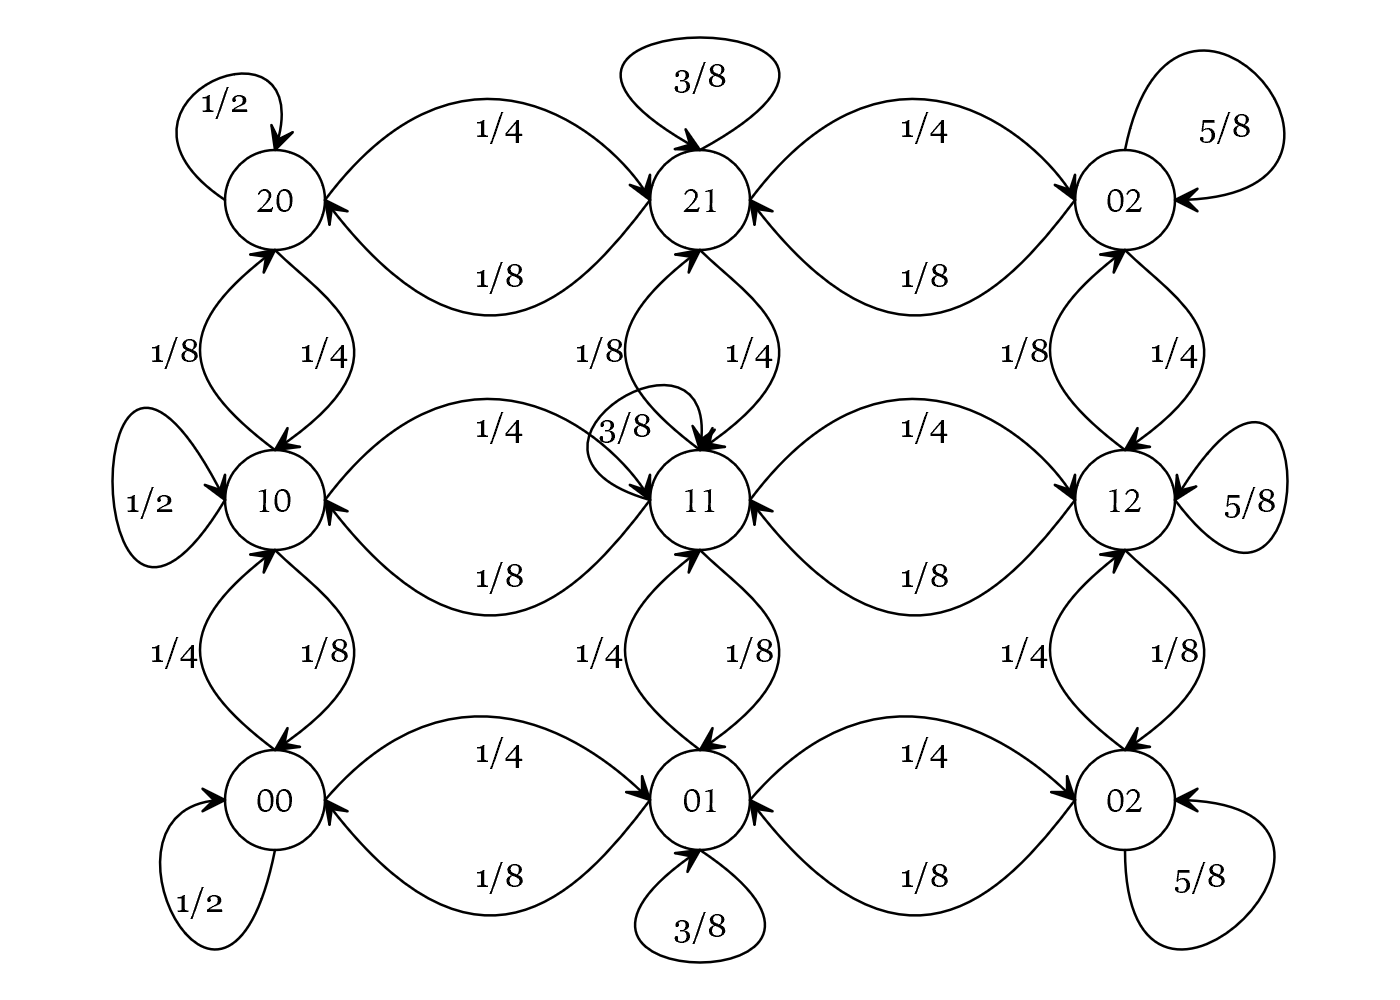
\includegraphics[width=350pt]{metro.png}
\caption{Metropolis-Hasting.}
\end{figure}

\section*{exercise 5.13}
\subsection*{(a)}

\begin{figure}[H]
	\centering
	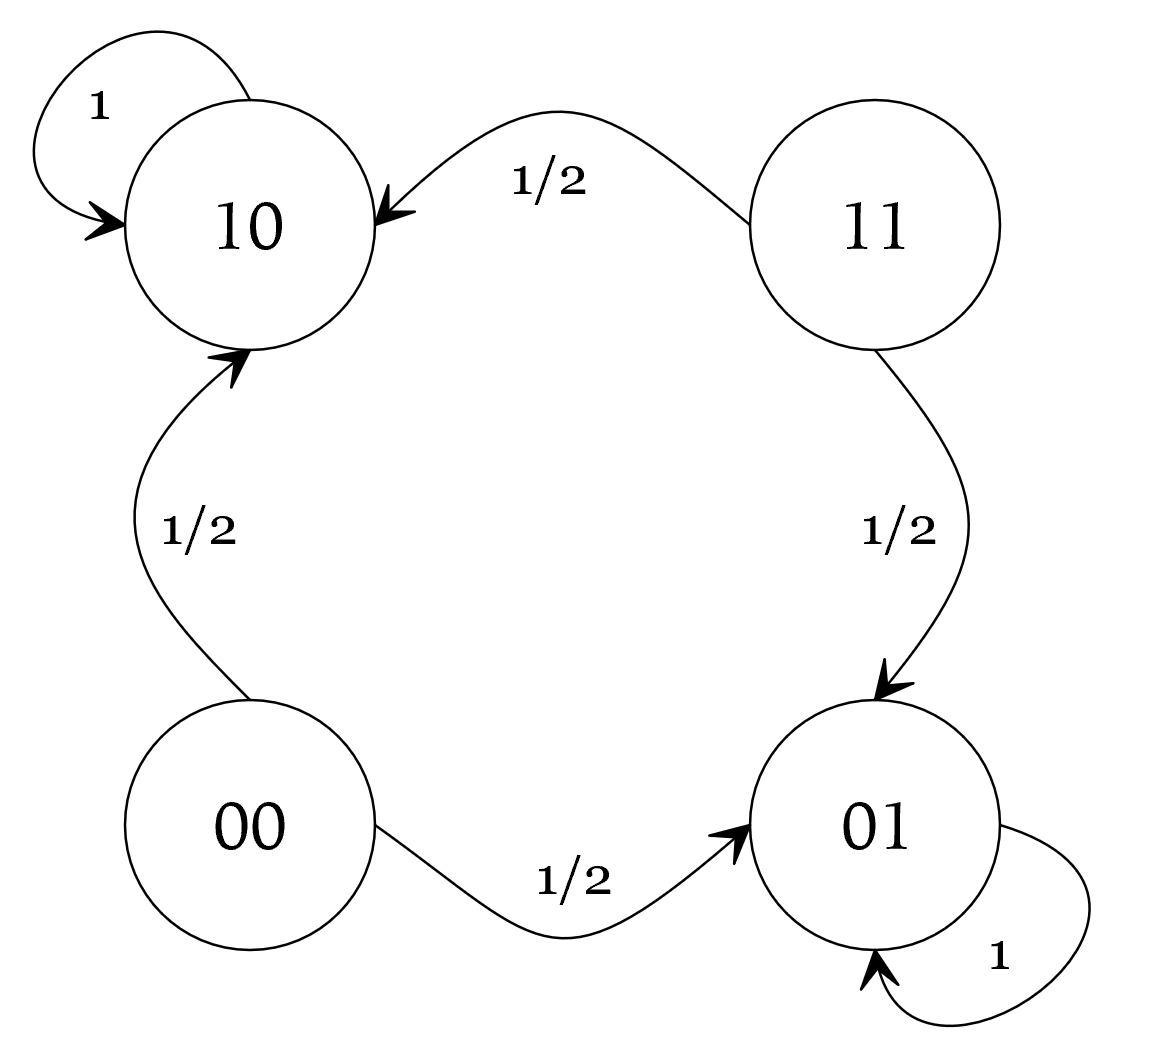
\includegraphics[width=350pt]{gibbs-13.png}
	\caption{Gibbs-Sampling.}
\end{figure}

\subsection*{(b)}

\begin{figure}[H]
	\centering
	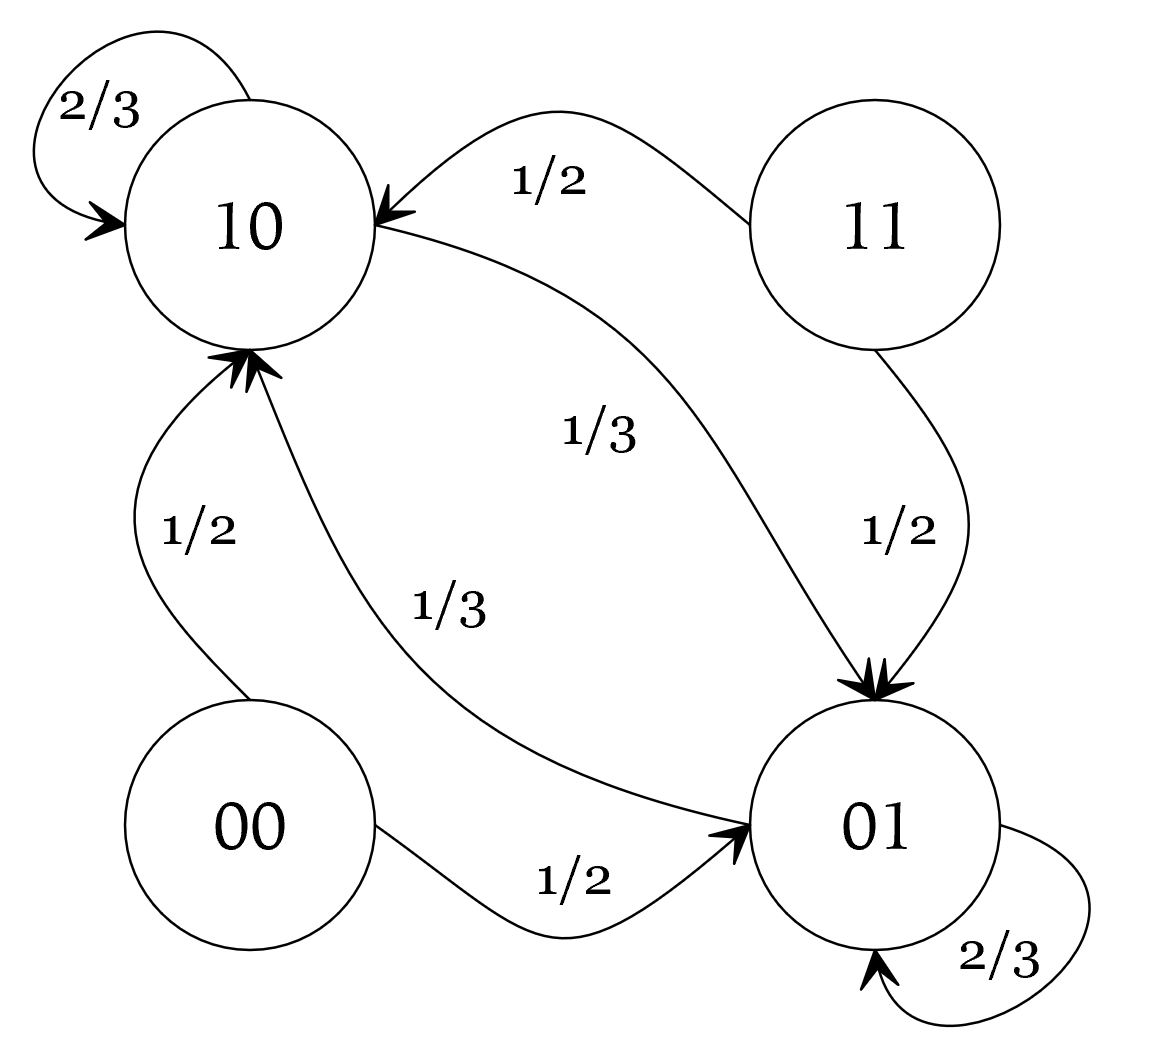
\includegraphics[width=350pt]{metro-13.png}
	\caption{Metropolis-Hasting.}
\end{figure}

\section*{exercise 5.16}
Construct a {\it Markov Chain} in the following way({\it Metropolis-Hasting Algorithm}):

\begin{eqnarray*}
V & = & {G \choose k} \\
d & = & k(n - k)  \\
p\left(S_1, S_2\right) & = & \left\{
\begin{array}{ll} 
\frac{1}{d} \max\left\{1, \frac{|E_{S_2}|}{|E_{S_1}|} \right\}& \left|S_1 \cap S_2\right| = k - 1\\ 
1 - \sum\limits_{S'\not= S_2} p(S_1, S') & S_1 = S_2 \\
0 & \textrm{otherwise} 
\end{array}\right. 
\end{eqnarray*}
In which $|E_S|$ is the number of edges in the subgraph induced on $S$.

\section*{exercise 5.18}
\subsection*{(a)}
Suppose the sizes of two cliques are $n$ and $m$ respectively($n > m$). Then the maximal degree $d = n + m$, use {\it Metropolis-Hasting Algorithm} to determine the transition probability $$p_{xy} = \frac{1}{d}\min\left\{1, \frac{\pi_y}{\pi_x}\right\} = \frac{1}{d}$$

Use $V$ to denote the vertex set of the graph, and $V_1, V_2$ to denote the vertex set of the two cliques, respectively. Let $S = S_1 \cup S_2, S_1 \subseteq V_1, S_2 \subseteq V_2, S_1 \cap S_2 = \emptyset$ be a subset of $V$ with $|S| = \left\lfloor \frac{n+m}{2} \right\rfloor$.

Suppose $v_1\in V_1$, $v_2\in V_2$ are connected. Compute $\Phi$ under different conditions:
\begin{description}
	\item[$v_1 \in S_1, v_2 \in S_2$:] $$\frac{1}{|S|} \left(|S_1|(n - |S_1|) + |S_2|(m - |S_2|)\right) \frac{1}{d}$$
	\item[$v_1 \not\in S_1, v_2 \in S_2$:] $$\frac{1}{|S|} \left(|S_1|(n - |S_1|) + |S_2|(m - |S_2|) + 1\right) \frac{1}{d}$$
	\item[$v_1 \in S_1, v_2 \not\in S_2$:] $$\frac{1}{|S|} \left(|S_1|(n - |S_1|) + |S_2|(m - |S_2|) + 1\right) \frac{1}{d}$$
	\item[$v_1 \not\in S_1, v_2 \not\in S_2$:] $$\frac{1}{|S|} \left(|S_1|(n - |S_1|)  + |S_2|(m - |S_2|)\right) \frac{1}{d}$$
\end{description}

In both cases, the minimal $\Phi$ is of order $O(\frac{n^2 + m^2}{(n+m)^2})$.

$$\varepsilon\textrm{-mixing time} =  O\left(\frac{\log \frac{1}{\pi_{min}}}{\Phi^2 \varepsilon^3}\right) = O\left(\frac{1}{\varepsilon^3}\frac{(n+m)^4}{(n^2 + m^2)^2} \log(n+m)\right)$$

\subsection*{(b)}
It's the same case as in the first question if we set the smaller clique's size as $1$:

$$\varepsilon\textrm{-mixing time} = O\left(\frac{1}{\varepsilon^3}\frac{(n+1)^4}{(n^2 + 1)^2} \log(n+m)\right) = O\left(\frac{1}{\varepsilon^3}\log(n+m)\right) $$
\section*{exercise 5.23}
Construct a circuit in the following way(Use the property $p_{xy} = \frac{C_{xy}}{C_x}$ to derive $R_{xy}$):

\begin{figure}[H]
	\centering
	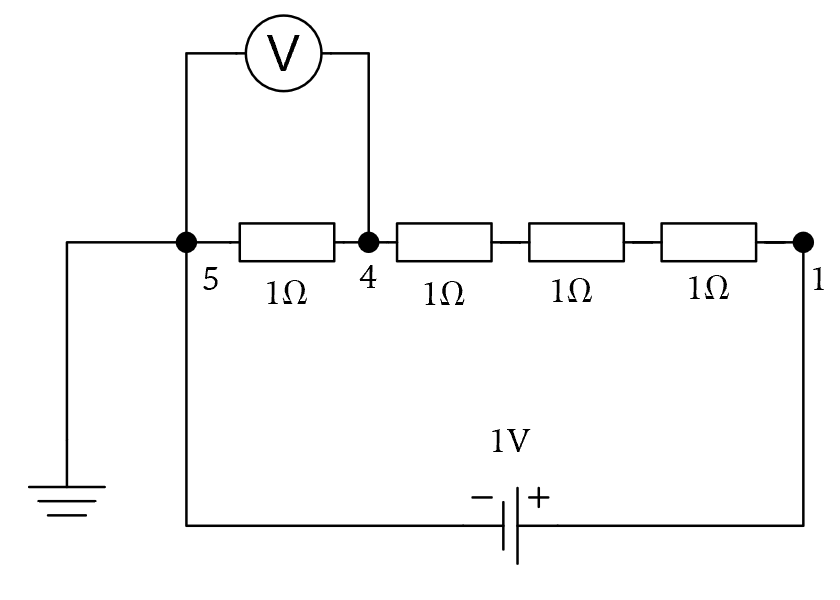
\includegraphics[width=350pt]{circuit.png}
	\caption{Circuit.}
\end{figure}

$$V_4 = \frac{1}{4} V $$

Thus the probability of a random walk starting at $4$ reaching $1$ before $5$ is $\frac{1}{4}$. 
\section*{exercise 5.44}
\subsection*{Description}
Prove that two independent random walks starting at the origin on a two dimensional lattice will eventually meet with probability one.
\subsection*{Solution}

Use $A$, $B$ to denote the two independent random walks. Suppose $B$'s position is fixed, then $A$'s move could be regarded as the graph showed below:

\begin{figure}[H]
	\centering
	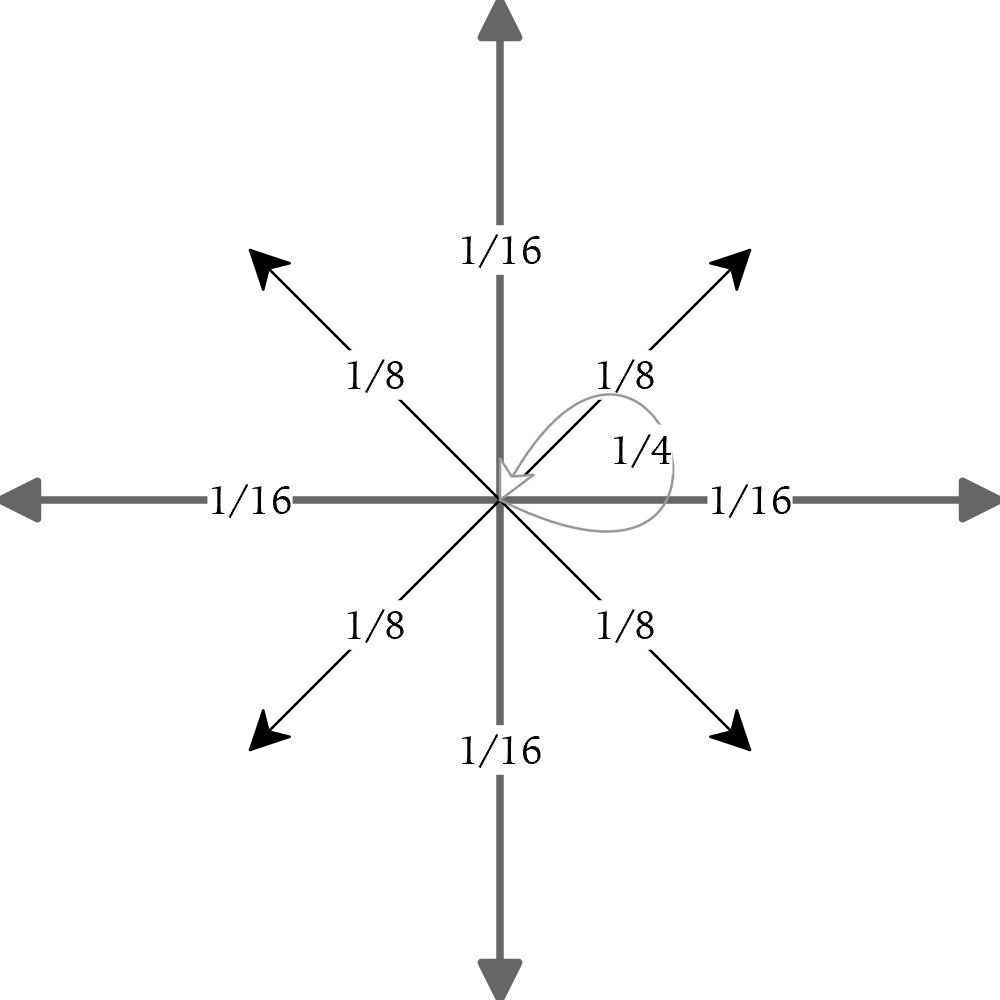
\includegraphics[width=350pt]{walk.png}
	\caption{Random Walk.}
\end{figure}

We just need to calculate the escape probability of $A$. However, the electrical circuit corresponding to this random walk is:

\begin{figure}[H]
	\centering
	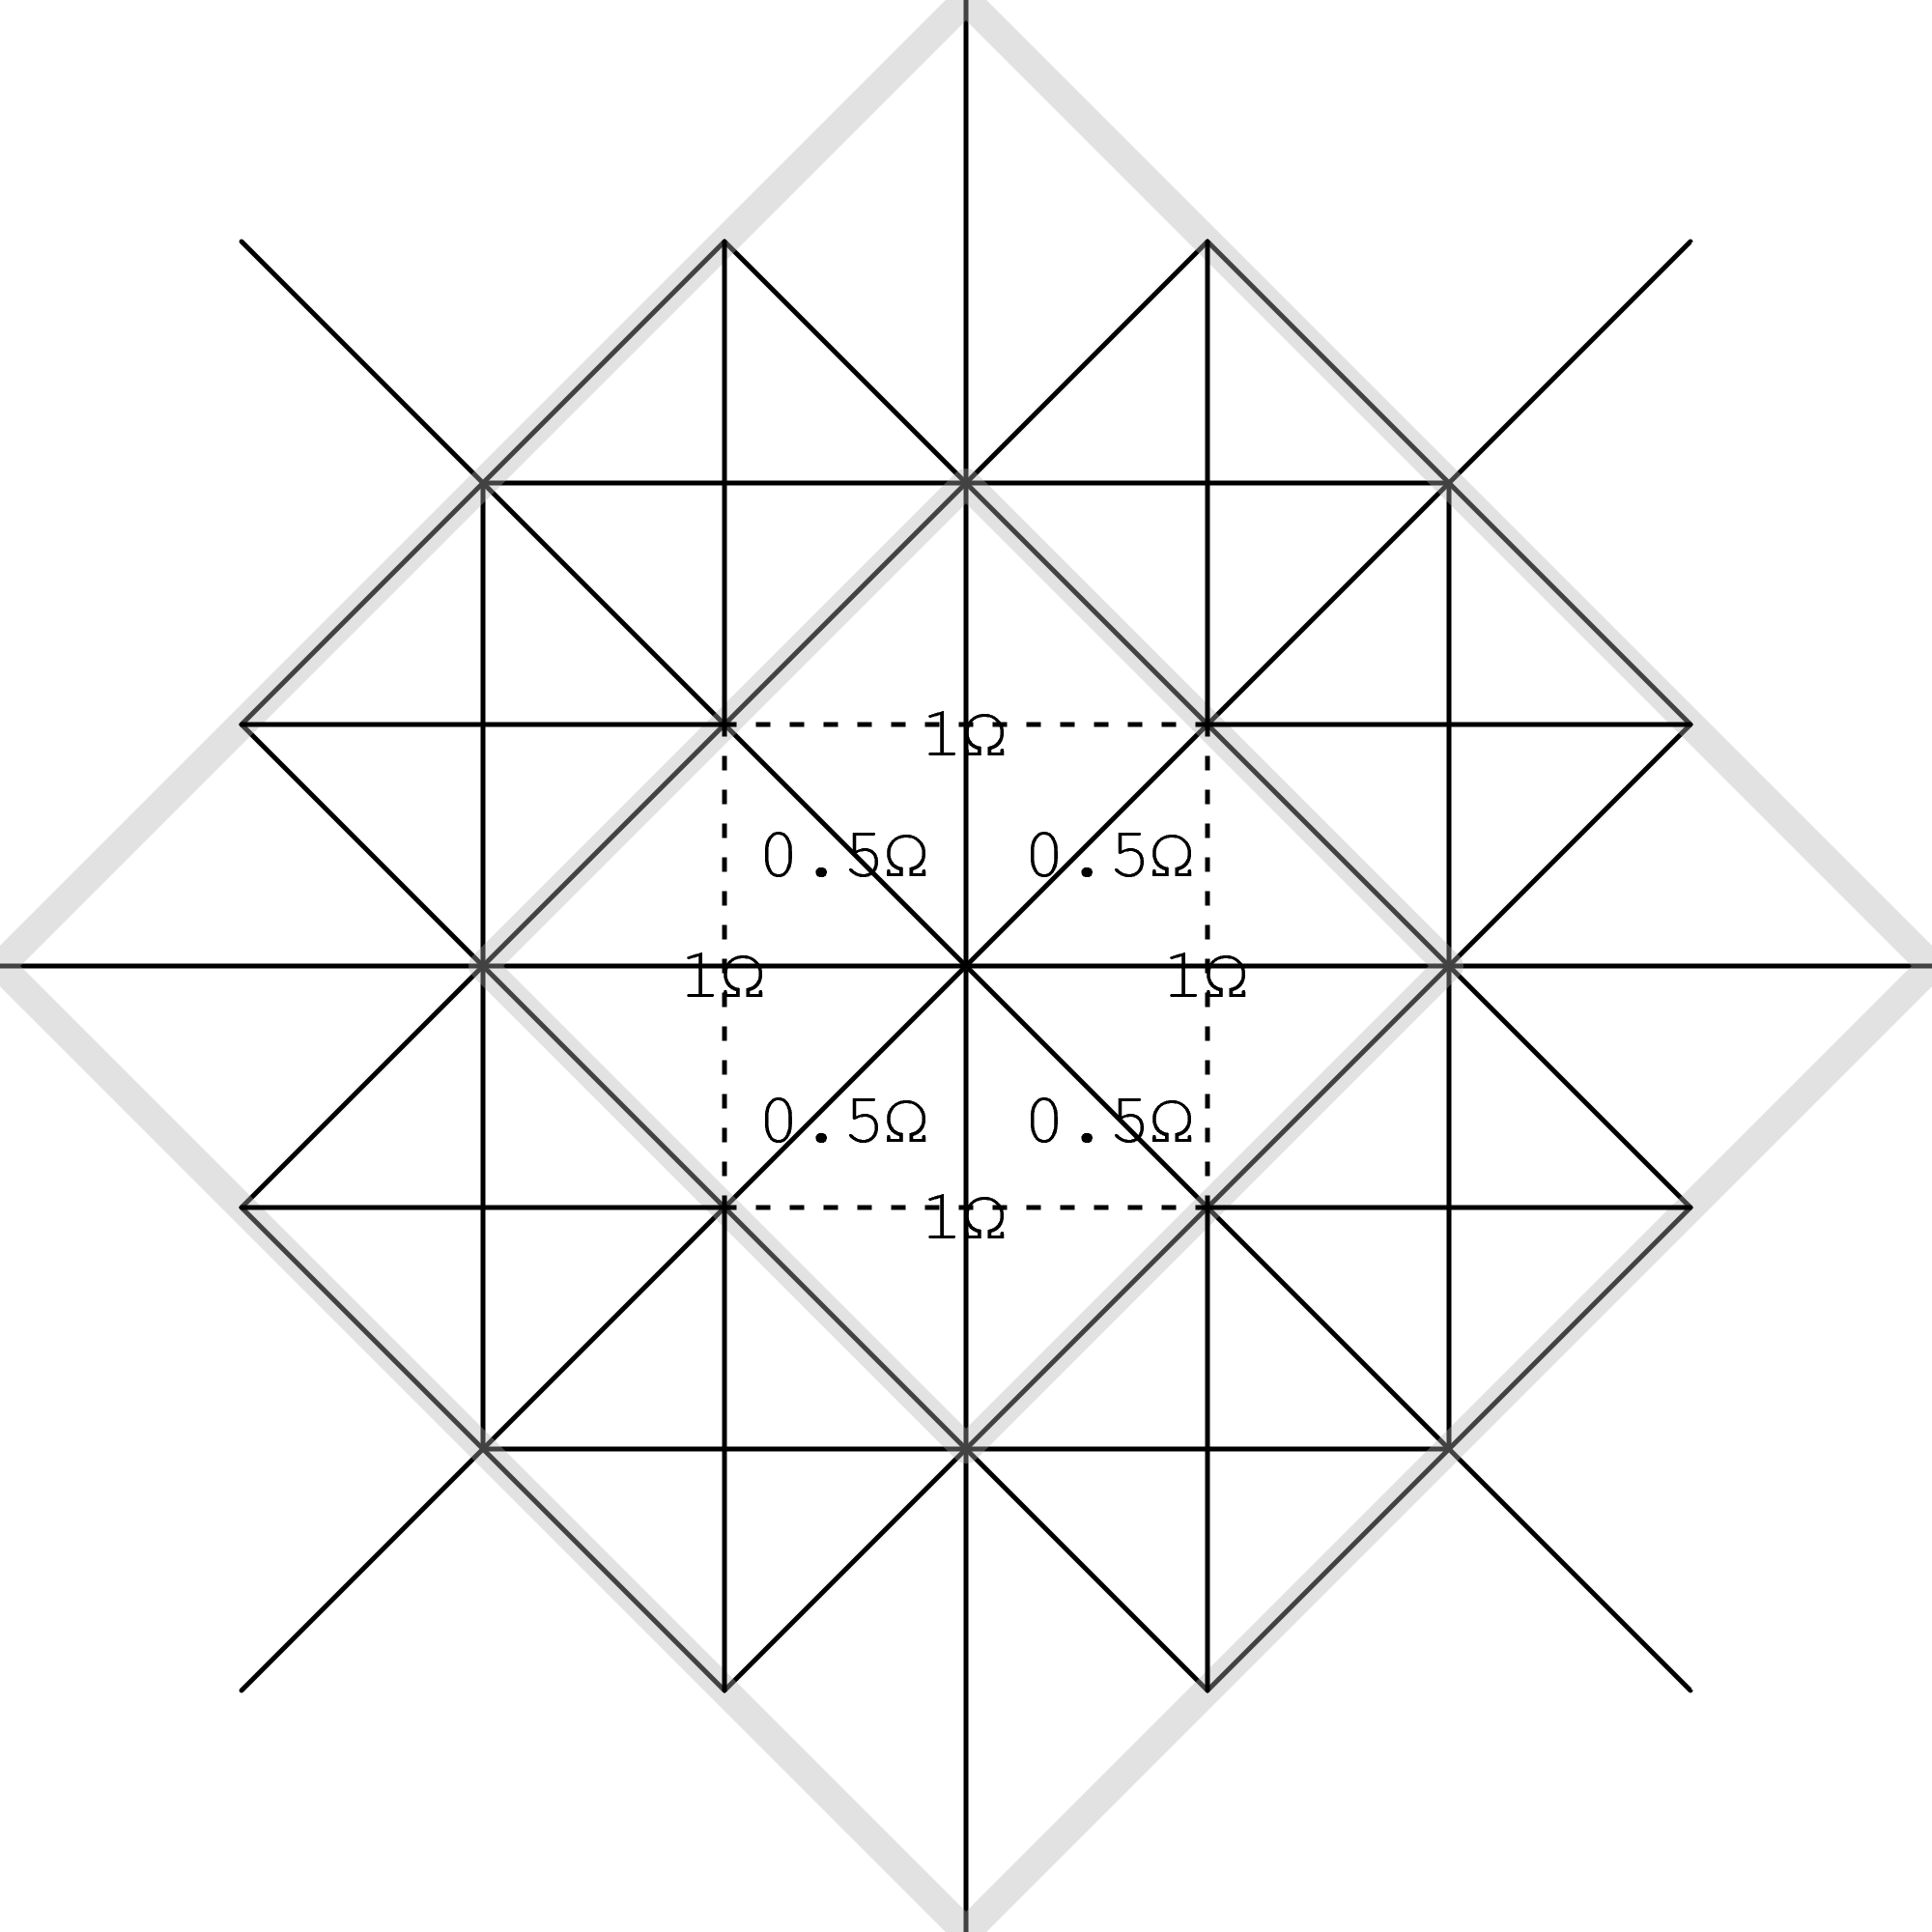
\includegraphics[width=350pt]{whole.png}
	\caption{Electrical Circuit.}
\end{figure}

Let $r_n$ be the resistance between $(0, 0)$ and the $n$-th boundary($|x| + |y| = n$), From the circuit we derive:

$$r_{n} \geq \frac{1}{12\Omega} + \sum_{i=2}^{n} \frac{1}{32i-20} $$ 

$$p_{escape} = \frac{c_{eff}}{c_a} = \frac{1}{16r_{eff}} = \lim_{n\to\infty}\frac{1}{\frac{4}{3} + \sum\limits_{i=2}^{n}\frac{4}{8i-5}} = 0$$
Thus with probability $1$, $A$ will return to the origin($A$), which implies $A$ will meet $B$ at some moment.
\end{document}